%ARQUIVO DE PREAMBULO DA TESE - PACOTES E CONFIGURA\c{C}\~{O}ES
%Version modified by Renan Moioli, 2014
\documentclass[
	% -- op\c{c}\~{o}es da classe memoir --
	12pt,				% tamanho da fonte
	openany,			% cap\'{\i}tulos come\c{c}am em p\'{a}g \'{\i}mpar (insere p\'{a}gina vazia caso preciso)
	oneside,			% para impress\~{a}o em verso e anverso. Oposto a oneside
	letterpaper,		% tamanho do papel.
	% -- op\c{c}\~{o}es da classe abntex2 --
	%chapter=TITLE,		% t\'{\i}tulos de cap\'{\i}tulos convertidos em letras mai\'{u}sculas
	%section=TITLE,		% t\'{\i}tulos de se\c{c}\~{o}es convertidos em letras mai\'{u}sculas
	%subsection=TITLE,	% t\'{\i}tulos de subse\c{c}\~{o}es convertidos em letras mai\'{u}sculas
	%subsubsection=TITLE,% t\'{\i}tulos de subsubse\c{c}\~{o}es convertidos em letras mai\'{u}sculas
	% -- op\c{c}\~{o}es do pacote babel --
	english,			% idioma adicional para hifeniza\c{c}\~{a}o
	french,			% idioma adicional para hifeniza\c{c}\~{a}o
	spanish,			% idioma adicional para hifeniza\c{c}\~{a}o
	brazil,				% o \'{u}ltimo idioma \'{e} o principal do documento
	sumario=tradicional,
	]{abntex2}

% ---
% PACOTES
% ---
%%%%%%%%%%%%%%%%%
\usepackage[utf8]{inputenc}
\usepackage[table]{xcolor}
% \usepackage[T1]{fontenc}
\usepackage{amsmath}
\usepackage{amsfonts}
\usepackage{algorithmic}
\usepackage[Algorithm]{algorithm}
\usepackage{textcomp}
%%%%%%%%%%%%%%%%%%
% ---
% Pacotes fundamentais
% ---
\usepackage[centerlast,small,sc]{caption} % Loaded by Thesis.cls
\usepackage{hyperref}                     % Loaded by Thesis.cls
\usepackage{epsfig}
%\usepackage{subfigure}
\usepackage{subcaption}
%\usepackage{algpseudocode}
\usepackage{cmap}				% Mapear caracteres especiais no PDF
\usepackage{lmodern}			% Usa a fonte Latin Modern			
\usepackage[T1]{fontenc}		% Selecao de codigos de fonte.
\usepackage[utf8]{inputenc}		% Codificacao do documento (convers\~{a}o autom\'{a}tica dos acentos)
\usepackage{lastpage}			% Usado pela Ficha catalogr\'{a}fica
\usepackage{indentfirst}		% Indenta o primeiro par\'{a}grafo de cada se\c{c}\~{a}o.
\usepackage{color}				% Controle das cores	% Inclus\~{a}o de gr\'{a}ficos
           % Pacote que converte as figuras em eps para pdf
\usepackage{lipsum}             % Pacote que gera texto dummy
\usepackage{blindtext}          % Pacote que gera texto dummy
\usepackage[utf8]{inputenc}
% ---
		
% ---
% Pacotes adicionais, usados apenas no \^{a}mbito do Modelo Can\^{o}nico do abnteX2
% ---
\usepackage{multirow}
\usepackage{rotating}
\usepackage{pdfpages}
% ---

% ---
% Pacotes de cita\c{c}\~{o}es
% ---
\usepackage[brazilian,hyperpageref]{backref}	 % Paginas com as cita\c{c}\~{o}es na bibl
\usepackage[alf,abnt-etal-cite=2,abnt-etal-list=0,abnt-etal-text=emph]{abntex2cite}	% Cita\c{c}\~{o}es padr\~{a}o ABNT

% ---
% Pacote de customiza\c{c}\~{a}o - Unicamp
% Modified by Moioli 2014
% ---
\usepackage{iinnels}


% ---
% CONFIGURA\c{C}\~{O}ES DE PACOTES
% ---

\counterwithin{figure}{chapter}
\counterwithin{table}{chapter}

% ---
% Configura\c{c}\~{o}es do pacote backref
% Usado sem a op\c{c}\~{a}o hyperpageref de backref
\graphicspath{{./figuras/}}
\DeclareGraphicsExtensions{.eps}

%customiza\c{c}\~{a}o do negrito em ambientes matem\'{a}ticos
\newcommand{\mb}[1]{\mathbf{#1}}
%customiza\c{c}\~{a}o de teoremas
\newtheorem{mydef}{Defini\c{c}\~{a}o}[chapter]
\newtheorem{lemm}{Lema}[chapter]
\newtheorem{theorem}{Teorema}[chapter]
\floatname{algorithm}{Pseudoc\'{o}digo}
\renewcommand{\listalgorithmname}{Lista de Pseudoc\'{o}digos}


\renewcommand{\backrefpagesname}{Citado na(s) p\'{a}gina(s):~}
% Texto padr\~{a}o antes do n\'{u}mero das p\'{a}ginas
\renewcommand{\backref}{}
% Define os textos da cita\c{c}\~{a}o
\renewcommand*{\backrefalt}[4]{
	\ifcase #1 %
		Nenhuma cita\c{c}\~{a}o no texto.%
	\or
		Citado na p\'{a}gina #2.%
	\else
		Citado #1 vezes nas p\'{a}ginas #2.%
	\fi}%
% ---


% ---
% Configura\c{c}\~{o}es de apar\^{e}ncia do PDF final

% alterando o aspecto da cor azul
\definecolor{blue}{RGB}{41,5,195}

% informa\c{c}\~{o}es do PDF
\makeatletter
\hypersetup{
     	%pagebackref=true,
		pdftitle={\@title},
		pdfauthor={\@author},
    	pdfsubject={\imprimirpreambulo},
	    pdfcreator={LaTeX with abnTeX2},
		pdfkeywords={abnt}{latex}{abntex}{abntex2}{trabalho acad\^{e}mico},
		hidelinks,					% desabilita as bordas dos links
		colorlinks=false,       	% false: boxed links; true: colored links
    	linkcolor=blue,          	% color of internal links
    	citecolor=blue,        		% color of links to bibliography
    	filecolor=magenta,      	% color of file links
		urlcolor=blue,
%		linkbordercolor={1 1 1},	% set to white
		bookmarksdepth=4
}
\makeatother
% ---

% ---
% Espa\c{c}amentos entre linhas e par\'{a}grafos
% ---

% O tamanho do par\'{a}grafo \'{e} dado por:
\setlength{\parindent}{1.3cm}

% Controle do espa\c{c}amento entre um par\'{a}grafo e outro:
\setlength{\parskip}{0.2cm}  % tente tamb\'{e}m \onelineskip

% ---
% Informacoes de dados para CAPA e FOLHA DE ROSTO
% Adaptado para IINN-ELS 
% ---
\titulo{T\'{\i}tulo da Qualifica\c{c}\~{a}o}
\autor{Autor}
\local{Macaíba}
\data{2020}
\orientador{Prof. Dr.}
\coorientador[Co-orientador]{Prof. Dr.}
\instituicao{%
    INSTITUTO INTERNACIONAL\\ DE NEUROCI\^{E}NCIAS\\ EDMOND E LILY SAFRA \\ Programa de P\'{o}s-Gradua\c{c}\~{a}o em Neuroengenharia}
%\tipotrabalho{Tese (Doutorado)}
%\preambulo{Tese apresentada ao Programa de P\'{o}s-Gradua\c{c}\~{a}o do Instituto Internacional de Neuroci\^{e}ncias de Natal - Edmond e Lily Safra como parte dos %requisitos exigidos para a obten\c{c}\~{a}o do t\'{\i}tulo de Doutor em Neuroengenharia.}
\tipotrabalho{Qualificação (Mestrado)}
\preambulo{Qualificação apresentada ao Programa de Pós Graduação em Neuroengenharia do Instituto Internacional de Neuroci\^{e}ncias - Edmond e Lily Safra como parte dos requisitos exigidos para a obten\c{c}\~{a}o do t\'{\i}tulo de Mestre em Neuroengenharia.}
% ---


%%%%%%%%%%%%%%%%
% Configuração da fonte -----------------------------------------------
% Não aparecer o número na primeira página dos capítulos
\newcommand{\mychapter}[1]{\chapter{#1}\thispagestyle{empty}}

% Os capítulos sem número
%\newcommand{\mychapterstar}[1]{\chapter*{#1}\thispagestyle{empty}}
\newcommand{\mychapterast}[1]{\chapter*{#1}\thispagestyle{empty}
\chaptermark{#1}
\afterpage{\markboth{\uppercase{#1}}{\rightmark}}
\markboth{\uppercase{#1}}{}
}

% Seções --------------------------------------------------------------------
% Seções sem número
\newcommand{\mysectionast}[1]{\section*{#1}
\addcontentsline{toc}{section}{#1}
\markright{\uppercase{#1}}
}

% Comandos matemáticos ---------------------------------------------------------
% Implicação em fórmulas
\newcommand{\implica}{\quad\Rightarrow\quad} %Meio de linha
\newcommand{\implicafim}{\quad\Rightarrow}   %Fim de linha
\newcommand{\tende}{\rightarrow}

% Fração com parenteses
\newcommand{\pfrac}[2]{\parent{\frac{#1}{#2}}}

% Transformada de Laplace e transformada Z
\newcommand{\lapl}{\pounds}
\newcommand{\transfz}{\mathcal{Z}}

% Sequências
\newcommand{\sequencia}[4]{$#1_{#2}$, $#1_{#3}$, \ldots, $#1_{#4}$}

% Teoremas
\newtheorem{thm}{Teorema}

% Senos e Cosenos
\newcommand{\sen}[1]{\text{sen}\left(#1\right)}
%\renewcommand{\cos}[1]{\text{cos}\left(#1\right)}

% Outros 
\newcommand{\jw}{j\omega}
\newcommand{\norm}[1]{\lVert#1\rVert_2}
\newcommand{\mbf}[1]{\mathbf{#1}}

% Tabelas ---------------------------------------------------------------------
% No tabularx, as celulas devem ser centradas verticalmente
\renewcommand{\tabularxcolumn}[1]{m{#1}}

% Células centralizadas horizontalmente no tabularx
\newcolumntype{C}{>{\centering\arraybackslash}X}

% Legendas ---------------------------------------------------------------------
% Abrevia figuras e tabelas
%\def\figurename{Fig.}
%\def\tablename{Tab.}

% Incluir fonte nas figuras e tabelas
\newcommand{\source}[1]{\vspace{3pt} \caption*{Fonte: {#1}}\vspace{-10pt} }

% Outros ----------------------------------------------------------------------
\newcommand{\chave}[1]{\left\{#1\right\}}
\newcommand{\colchete}[1]{\left[#1\right]}
\newcommand{\parent}[1]{\left(#1\right)}

% Paths

\everymath{\displaystyle}

%%%%%%%%%%%%%%%%

\makeindex
\usepackage{nomencl}
\makenomenclature
\usepackage{float}
\usepackage{hyperref}
\usepackage{amsmath}

\begin{document}
% Retira espaço extra obsoleto entre as frases.
\frenchspacing
% ---- ELEMENTOS PRÉ-TEXTUAIS ----
\pretextual

\pagenumbering{roman}\author{AUTOR}
\title{TÍTULO}

\imprimircapa

\setcounter{page}{2} \imprimirfolhaderosto* % Folha de rosto (o * indica que haverá ficha catalográfica) 
{\color{white}\rule{\linewidth}{0.5mm} } 

%%Isto \'{e} um exemplo de Ficha Catalogr\'{a}fica, ou ``Dados internacionais de
%cataloga\c{c}\~{a}o-na-publica\c{c}\~{a}o''. Voc\^{e} pode utilizar este modelo como refer\^{e}ncia.
%Por\'{e}m, provavelmente a biblioteca da sua universidade lhe fornecer\'{a} um PDF
%com a ficha catalogr\'{a}fica definitiva ap\'{o}s a defesa do trabalho. Quando estiver
%com o documento, salve-o como PDF no diret\'{o}rio do seu projeto e substitua todo
%o conte\'{u}do de implementa\c{c}\~{a}o deste arquivo pelo comando abaixo:


    \begin{fichacatalografica}
    	\vspace*{\fill}					% Posição vertical
    	\hrule							% Linha horizontal
    	\begin{center}					% Minipage Centralizado
        	\begin{minipage}[c]{12.5cm}		% Largura
        	
            	\imprimirautor
            	
            	\hspace{0.5cm} \imprimirtitulo  / \imprimirautor. --
            	\imprimirlocal, \imprimirdata-
            	
            	\hspace{0.5cm} \pageref{LastPage} p. : il. (algumas color.) ; 30 cm.\\
            	
            	\hspace{0.5cm} \imprimirorientadorRotulo~\imprimirorientador\\
            	\hspace{0.5cm}
            	\parbox[t]{\textwidth}{\imprimirtipotrabalho~--~ INSTITUTO INTERNACIONAL DE NEUROCIÊNCIAS EDMOND E LILY SAFRA \\ Programa de Pós-Graduação em Neuroengenharia,
            	\imprimirdata.}\\
            	
            	\hspace{0.5cm}
            		1. Palavra-chave1.
            		2. Palavra-chave2.
            		I. Renan Cipriano Moioli.
            		II. Universidade xxx.
            		III. Faculdade de xxx.
            		IV. Título\\ 			
            	
            	\hspace{8.75cm} CDU 02:141:005.7\\
        	
        	\end{minipage}
    	\end{center}
    	\hrule
    \end{fichacatalografica}
    \setcounter{page}{3}
%%Isto \'{e} um exemplo de Folha de aprova\c{c}\~{a}o, elemento obrigat\'{o}rio da NBR
%14724/2011 (se\c{c}\~{a}o 4.2.1.3). Voc\^{e} pode utilizar este modelo at\'{e} a aprova\c{c}\~{a}o
%do trabalho. Ap\'{o}s isso, substitua todo o conte\'{u}do deste arquivo por uma
%imagem da p\'{a}gina assinada pela banca com o comando abaixo:

%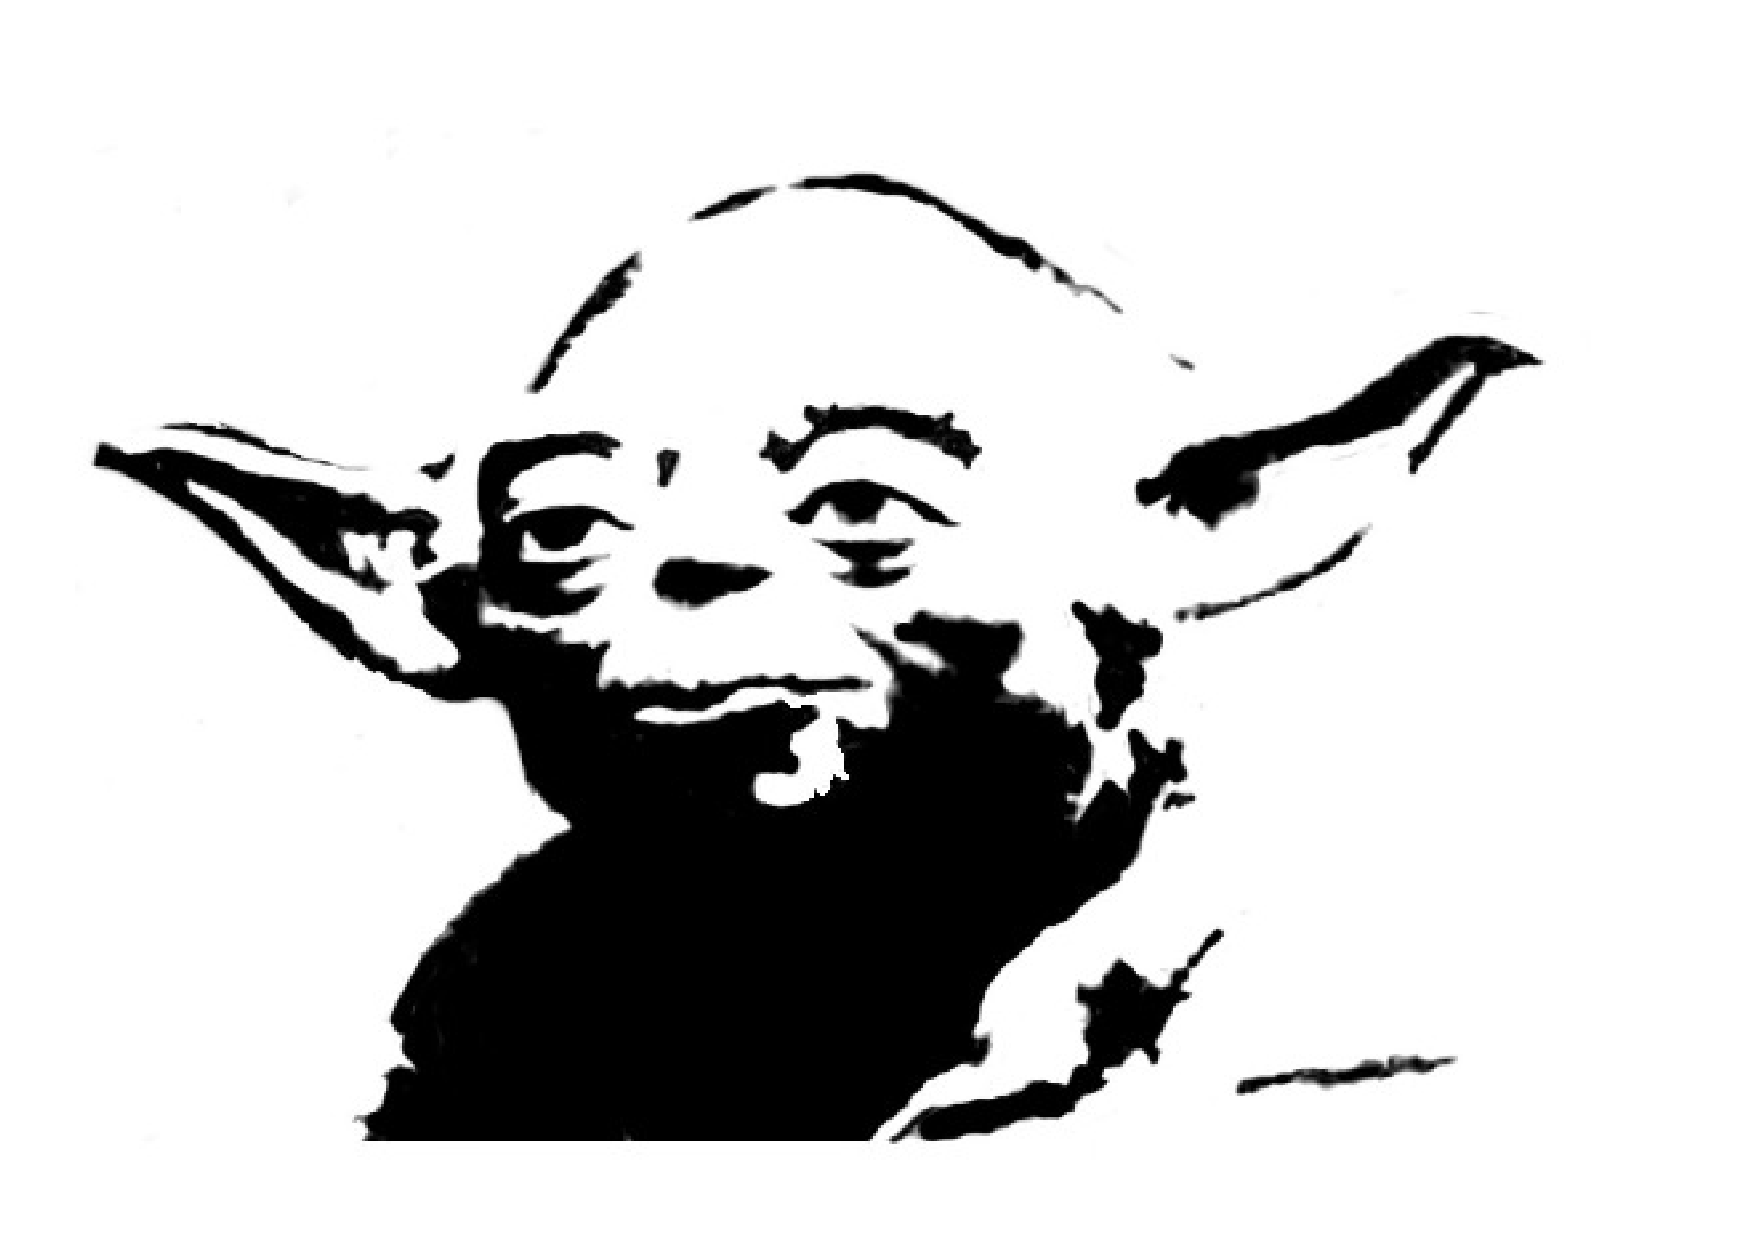
\includepdf[scale=0.3]{pretextual/folhadeaprovacao_final.pdf}

\begin{folhadeaprovacao}

  \begin{center}
    {\ABNTEXchapterfont\large\imprimirautor}

    \vspace*{\fill}\vspace*{\fill}
    \begin{center}
      \ABNTEXchapterfont\bfseries\Large\imprimirtitulo
    \end{center}
    \vspace*{\fill}
    
    \hspace{.45\textwidth}
    \begin{minipage}{.5\textwidth}
        \imprimirpreambulo
    \end{minipage}%
    \vspace*{\fill}
    \end{center}
        
    Trabalho aprovado. \imprimirlocal, 01 de Janeiro de 2015:

    \assinatura{\textbf{\imprimirorientador} \\} 
    \assinatura{\textbf{Professor} \\ Convidado 1}
    \assinatura{\textbf{Professor} \\ Convidado 2}
    %\assinatura{\textbf{Professor} \\ Convidado 3}
    %\assinatura{\textbf{Professor} \\ Convidado 4}
      
    \begin{center}
    \vspace*{0.5cm}
    {\large\imprimirlocal}
    \par
    {\large\imprimirdata}
    \vspace*{1cm}
  \end{center}
  
\end{folhadeaprovacao}
\begin{resumo}

%pode apagar!
Para alterar este texto basta dar um 
\textbf{duplo clique “aqui”}, e o local de edição será aberto na sua caixa de edição do lado “esquerdo”.

%pode apagar!
\textbf{Copie e cole seu texto aqui}

%Para retirar o negrito do texto utilize apenas \textf{ }
    \noindent\textbf{Palavras-chave}: xxxxxx; xxxxxx; xxxxxxxx.
\end{resumo}

\begin{otherlanguage*}{english}
    \begin{center}{\ABNTEXchapterfont\huge Abstract}\end{center}
%pode apagar!
Para alterar este texto basta dar um 
\textbf{duplo clique “aqui”}, e o local de edição será aberto na sua caixa de edição do lado “esquerdo”.

%pode apagar!
\textbf{Copie e cole seu texto aqui.}


    \vspace{\onelineskip}
    \noindent\textbf{Keywords}: xxxxxxxx; xxxxxxxx; xxxxxxxxxx.

\end{otherlanguage*} % --- RESUMOS (em portugu\^{e}s e ingl\^{e}s ---
\pdfbookmark[0]{\contentsname}{toc}
\tableofcontents*
\cleardoublepage
%\begin{dedicatoria}
    \vspace*{\fill}
    \centering
    \noindent
    \textit{Dedico esta tese \`{a} George Lucas.}
    \vspace*{\fill}
\end{dedicatoria}
%\begin{agradecimentos}
    \lipsum[1-3]
\end{agradecimentos}
%\begin{epigrafe}
    \vspace*{\fill}
	\begin{flushright}
		\textit{``Don't be too proud of this technological terror you've constructed. The ability to destroy a planet is insignificant next to the power of the Force.'' D.V.}
	\end{flushright}
\end{epigrafe}
\pdfbookmark[0]{\listfigurename}{lof}
\listoffigures*
\cleardoublepage
%\pdfbookmark[0]{\listtablename}{lot}
\listoftables*
\cleardoublepage
\renewcommand{\nomname}{Lista de Acr\^{o}nimos e Abrevia\c{c}\~{o}es}
\pdfbookmark[0]{\nomname}{las}
\printnomenclature
\cleardoublepage

\pagenumbering{arabic} \textual % ---- ELEMENTOS TEXTUAIS ----

\chapter[Introdução]{Introdução}

\textbf{Ler com bastante atenção:}

Alguns \textbf{manuais}, \textbf{exemplos} e \textbf{vídeos} de pacotes latex foram adicionados no capítulo \textbf{\ref{cap:cap01}}.

Todo o documento já está formatado com o layout utilizado pelo IIN-ELS. Você precisa apenas inserir as informações do seu trabalho nos respectivos tópicos.
É importante lembrar que todos os capítulos, subcapítulos e suas seções contidas aqui, são apenas exemplos, não sendo obrigatório para a sua qualificação/dissertação. Confiram os itens obrigatórios no documento "Normativa do Exame de Qualificação do Mestrado Acadêmico em Neuroengenharia".

Procure se informar a respeito do Mendeley. É um software para gerenciar referencias bibliográficas que irá facilitar muito a inclusão das referências no documento. Procure também como importar as referencias inseridas no mendeley para o arquivo references.bib aqui no overleaf.

Este documento e seu código-fonte são exemplos de referência de uso da classe \textsf{abntex2} e do pacote \textsf{abntex2cite}. O documento exemplifica a elaboração de trabalho acadêmico (tese, dissertação e outros do gênero) produzido conforme a ABNT NBR 14724:2011 \emph{Informação e documentação - Trabalhos acadêmicos - Apresentação}.

A expressão ``Modelo Canônico'' é utilizada para indicar que \abnTeX\ não é modelo específico de nenhuma universidade ou instituição, mas que implementa tão somente os requisitos das normas da ABNT. Uma lista completa das normas observadas pelo \abnTeX\ é apresentada em \citeonline{abntex2classe}. 

Este documento deve ser utilizado como complemento dos manuais do \abnTeX\ \cite{abntex2classe,abntex2cite,abntex2cite-alf} e da classe \textsf{memoir} \cite{memoir}.

%pode apagar!
Para alterar este texto basta dar um 
\textbf{duplo clique “aqui”}, e o local de edição será aberto na sua caixa de edição do lado “esquerdo”.

%pode apagar!
\textbf{Copie e cole seu texto aqui.}


\section{Justificativa}
	%pode apagar!
Para alterar este texto basta dar um 
\textbf{duplo clique “aqui”}, e o local de edição será aberto na sua caixa de edição do lado “esquerdo”.

%pode apagar!
\textbf{Copie e cole seu texto aqui.}


\section{Delimitação do tema ou problema}
    %pode apagar!
Para alterar este texto basta dar um 
\textbf{duplo clique “aqui”}, e o local de edição será aberto na sua caixa de edição do lado “esquerdo”.

%pode apagar!
\textbf{Copie e cole seu texto aqui.}


\section{Delimitação do trabalho}

%pode apagar!
Para alterar este texto basta dar um 
\textbf{duplo clique “aqui”}, e o local de edição será aberto na sua caixa de edição do lado “esquerdo”.

%pode apagar!
\textbf{Copie e cole seu texto aqui.}

\section{Objetivos}

%pode apagar!
Para alterar este texto basta dar um 
\textbf{duplo clique “aqui”}, e o local de edição será aberto na sua caixa de edição do lado “esquerdo”.

%pode apagar!
\textbf{Copie e cole seu texto aqui.}

\subsection{Objetivos Gerais}
	
	%pode apagar!
Para alterar este texto basta dar um 
\textbf{duplo clique “aqui”}, e o local de edição será aberto na sua caixa de edição do lado “esquerdo”.

%pode apagar!
\textbf{Copie e cole seu texto aqui.}

    
\subsection{Objetivos Específicos}
    %pode apagar!
Para alterar este texto basta dar um 
\textbf{duplo clique “aqui”}, e o local de edição será aberto na sua caixa de edição do lado “esquerdo”.

%pode apagar!
\textbf{Copie e cole seu texto aqui.}

\chapter{Exemplo de Capítulo}
\label{cap:cap01}
%pode apagar!
Para alterar este texto basta dar um 
\textbf{duplo clique “aqui”}, e o local de edição será aberto na sua caixa de edição do lado “esquerdo”.

%pode apagar tudo!
\textbf{Copie e cole seu texto aqui.}

* Pretextual - nesta pasta estão contidos os arquivos relacionados aos resumo, agradecimentos, capa, dedicatória, epígrafe, ficha catalográfica, folha de aprovação, listas e sumário.

* figuras - todas as figuras do documento estarão contidas na pasta figuras.

* chapter - nesta pasta devem estar contidos todos os arquivos que compõe o texto da dissertação como a introdução,  referencial teórico, metodologia, resultados, discussão e conclusão.

* postextuais - nesta pasta devem estar contidos os arquivos dos elementos pós-textuais, ou seja, apêndices e anexos.

 O arquivo mais importante deste conjunto de arquivos que formam a dissertação é o "main.tex". Este arquivo é responsável por concentrar todos os outros e permitir que a compilação seja realizada adequadamente. Caso haja a necessidade do usuário adicionar novos elemetos pré, pós ou textuais, eles devem ser incluídos na sequência correta dentro do arquivo main.tex. Uma observação importante a ser realizada é que não há a necessidade de modificar o arquivo main exceto que o usuário deseje adicionar novos arquivos ao texto.

 Algumas considerações adicionais são importantes ao trabalhar com textos feitos em Latex, e, por isso, seria interessante fundamentar o conhecimento com alguns assuntos básicos a respeito da padronização de arquivos com o Latex:
 
 * Importância do Latex: \url{https://www.youtube.com/watch?v=QCEqv7wMmIg}

* Criando o primeiro Texto: \url{https://www.youtube.com/watch?v=Bivw_raoaz4}

* Segmentando o texto em arquivos: \url{https://www.youtube.com/watch?v=LXWOazgNqK4}

* Criando sistema de bibliografias: \url{https://www.youtube.com/watch?v=oztGf4m9vl8}

* Formatando figuras: \url{https://www.youtube.com/watch?v=0Lesgsa6zLw}

* Criando Tabelas: \url{https://www.youtube.com/watch?v=Q6H67XU1zuc}

* Criando Equações: \url{https://www.youtube.com/watch?v=aH-GmAZSoSg}

* Criando itens e enumeração: \url{https://www.youtube.com/watch?v=Ibj9wqCNNAg}

É importante lembrar que as explicações de cada tema levam em consideração a sua aplicação imediata em um documento com formatação básica. Porém, todo o conteúdo pode ser aplicado conceitualmente ao documento atual e, no caso das figuras, tabelas, equações e itens, o conteúdo pode e deve ser aplicado em cada arquivo dos elementos de texto contidos neste projeto.

\section{Exemplo de Subseção  de Capítulo}
\label{cap01:sec02}
%pode apagar!
Para alterar este texto basta dar um 
\textbf{duplo clique “aqui”}, e o local de edição será aberto na sua caixa de edição do lado “esquerdo”.

%pode apagar tudo!
\textbf{Copie e cole seu texto aqui.}

A formatação usada  pelas Normas ABNTex2 são:

\textbf{Papel}: A4 – cor branca

\textbf{Fonte}: Times New Roman ou Arial- tamanho 12 – cor: preta. Nas citações com mais de 3 linhas, notas de rodapé, legendas e tabelas a fonte deve ter o tamanho 10.

\textbf{Itálico}: Deve ser usado nas palavras de outros idiomas. Esta orientação não se aplica às expressões latinas apud e et al.

\textbf{Margens}: Direita e inferior: 2cm / Esquerda e superior: 3cm
Parágrafos / Espaçamento: 1,5 entre linhas;

As referências devem ser separadas umas das outras com espaçamento duplo.

\textbf{Alinhamento do texto}: O texto do trabalho deve estar justificado para que fique alinhado às margens esquerda e direita. Esta formatação revela uma aparência mais organizada e o escrito fica melhor distribuído.
\mychapter{Metodologia}

%pode apagar!
Para alterar este texto basta dar um 
\textbf{duplo clique “aqui”}, e o local de edição será aberto na sua caixa de edição do lado “esquerdo”.

%pode apagar tudo!
\textbf{Copie e cole seu texto aqui.}

\textbf{Para mudar a imagem basta alterar o caminho contido no comando "linewidth ${figuras/abntex2-modelo-img-grafico.pdf}$" para a imagem desejada.}

\textbf{OBS: todas as imagens devem ser colocadas na pasta figures, para isso basta clicar na pasta e clicar no botão Upload localizado no menu superior a esquerda. 
}

\begin{figure}[H]
\begin{center}
\caption{EXEMPLO DE FIGURA - TODO ESCRITO EM CAIXA ALTA.}
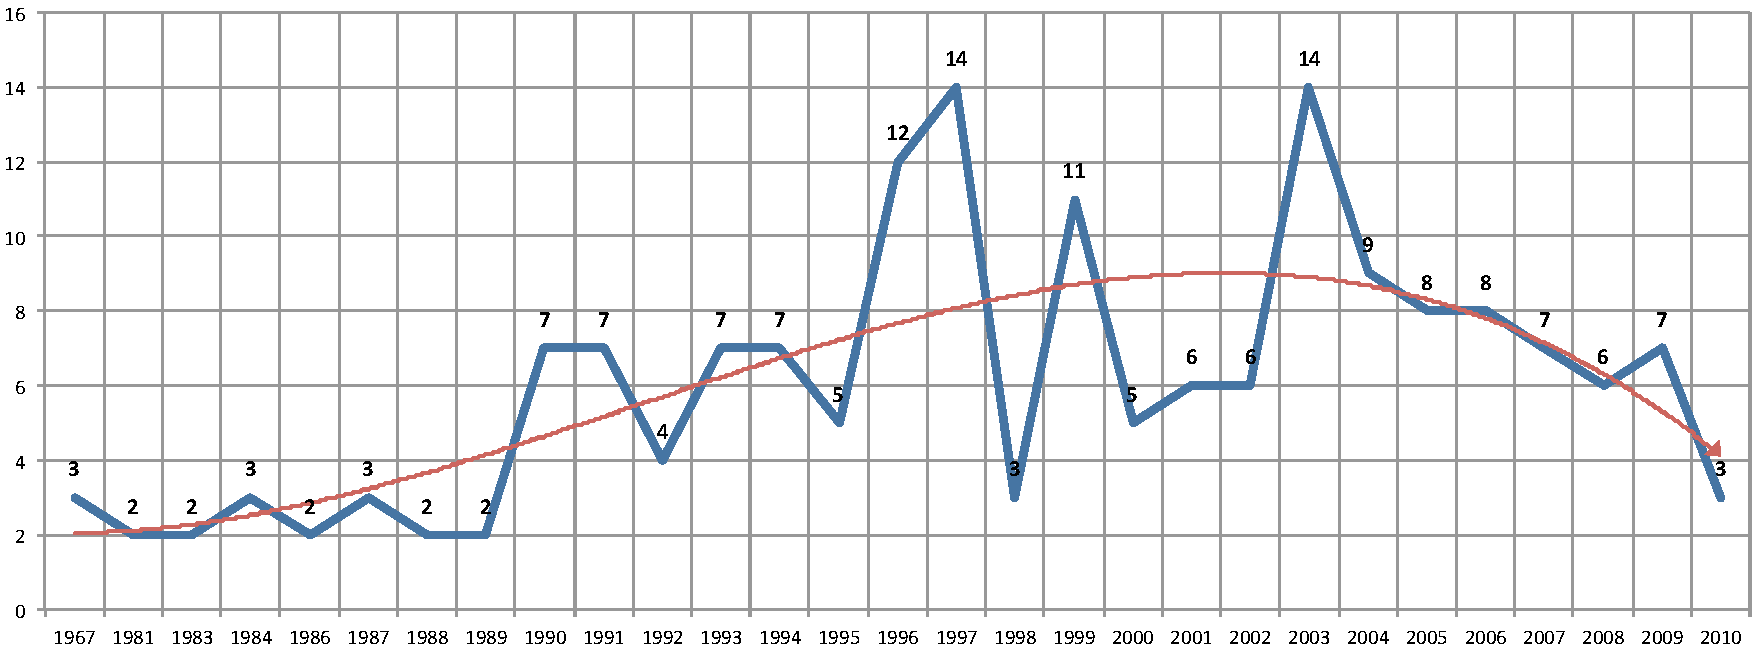
\includegraphics[width=12cm]{figuras/abntex2-modelo-img-grafico.pdf}
\legend{Fonte: Adaptado de \citeonline{NBR14724:2011}.}
\label{fig:controleUComparativo}
\end{center}
\end{figure}


\mychapter{Resultados Parciais}

%pode apagar!
Para alterar este texto basta dar um 
\textbf{duplo clique “aqui”}, e o local de edição será aberto na sua caixa de edição do lado “esquerdo”.

%pode apagar tudo!
\textbf{Copie e cole seu texto aqui.}

\begin{figure}[H]
\begin{center}
\caption{EXEMPLO DE FIGURA}
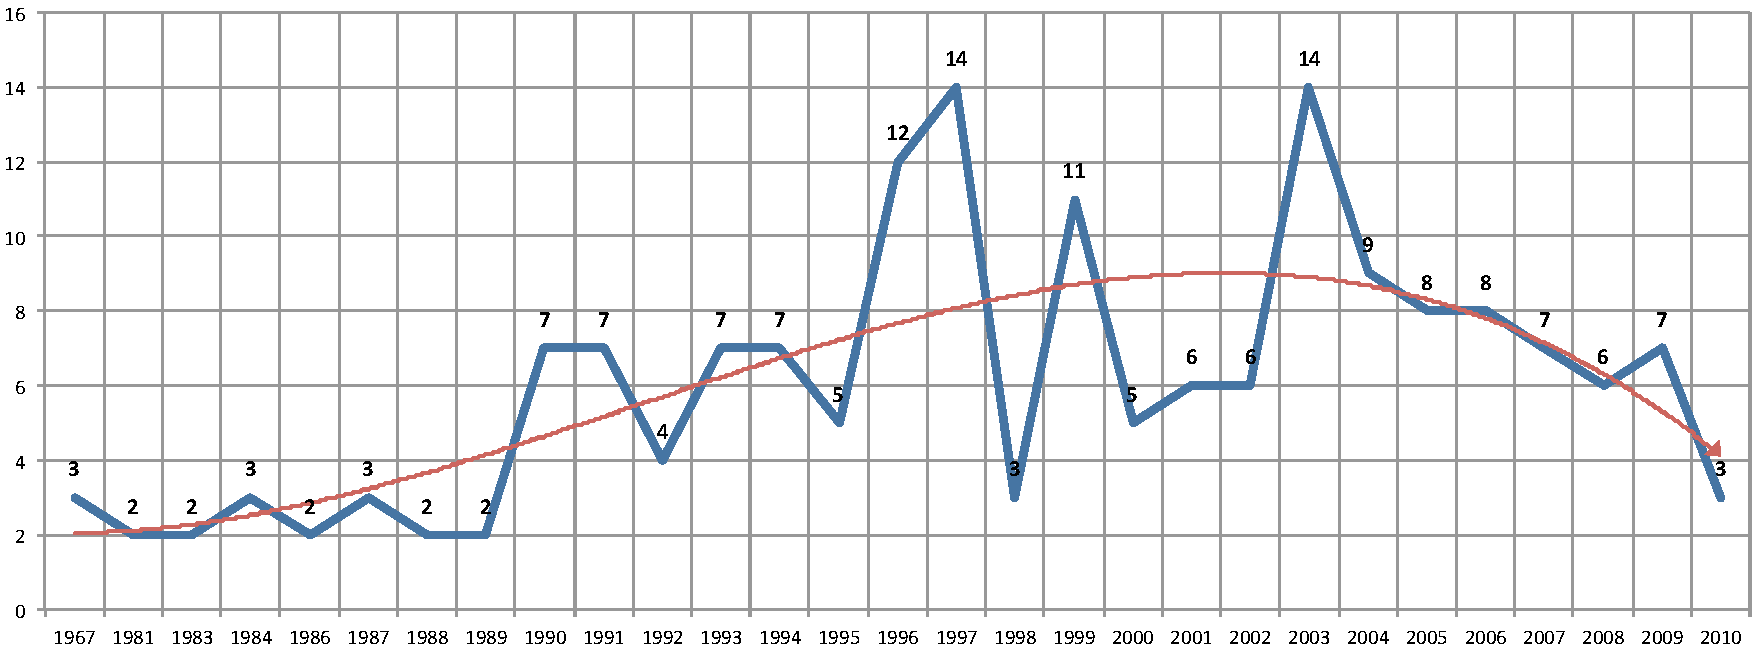
\includegraphics[width=12cm]{figuras/abntex2-modelo-img-grafico.pdf}
\legend{Fonte: Adaptado de \citeonline{NBR14724:2011}.}
\label{fig:Yoriginal}
\end{center}
\end{figure}

\bookmarksetup{startatroot}%% Finaliza a parte no bookmark do PDF, para que se inicie o bookmark na raiz 

\chapter[Conclusão]{Conclusão}
%pode apagar!
Para alterar este texto basta dar um 
\textbf{duplo clique “aqui”}, e o local de edição será aberto na sua caixa de edição do lado “esquerdo”.

%pode apagar tudo!
\textbf{Copie e cole seu texto aqui.}


\section{Trabalhos futuros}

%pode apagar!
Para alterar este texto basta dar um 
\textbf{duplo clique “aqui”}, e o local de edição será aberto na sua caixa de edição do lado “esquerdo”.

%pode apagar tudo!
\textbf{Copie e cole seu texto aqui.}
\chapter{Cronograma}

%pode apagar!
Para alterar este texto basta dar um 
\textbf{duplo clique “aqui”}, e o local de edição será aberto na sua caixa de edição do lado “esquerdo”.

%pode apagar tudo!
\textbf{Copie e cole seu texto aqui.}

\textbf{OBS: Crie sua tabela utilizando o seguinte site: \url{https://www.tablesgenerator.com}, Basta substituir a tabela abaixo pelo código latex gerado no site.}

A Tabela \ref{tab_cronograma} apresenta o cronograma de execução das atividades desta proposta.\\

\begin{table}[!htpb]
\centering
\caption{Cronograma das atividades previstas}
\setlength{\tabcolsep}{5pt} 
\begin{tabular}{|c|c|c|c|c|c|c|c|c|c|c|c|c|c|}\hline
 & \multicolumn{12}{c|}{Meses}\\ \cline{2-13}
\raisebox{1.5ex}{Etapa} & 1 & 2 & 3 & 4 & 5 & 6 & 7 & 8 & 9 & 10 & 11 & 12 \\ \hline \hline
A1 & \cellcolor{black} &   &   &   &   &   &   &   &   &   &   &   \\ \hline
A2 &   & \cellcolor{black} &   &   &   &   &   &   &   &   &   &   \\ \hline
A3 &   & \cellcolor{black} & \cellcolor{black} &   &   &   &   &   &   &   &   &   \\ \hline
A4 &   &   &   & \cellcolor{black} & \cellcolor{black} &   &   &   &   &   &   &   \\ \hline
A5 &   &   &   &   &   & \cellcolor{black} & \cellcolor{black} &   &   &   &   &   \\ \hline
A6 &   &   &   &   &   &   &   & \cellcolor{black} & \cellcolor{black} &   &   &   \\ \hline
A7 &   &   &   &   &   &   &   &   &   & \cellcolor{black} & \cellcolor{black} & \cellcolor{black} \\ \hline
\end{tabular} 
\legend{Fonte: Produzido pelo autor  }
\label{tab_cronograma}
\end{table}
% ---- ELEMENTOS P\'{O}S-TEXTUAIS ----
\postextual

\bibliography{references}
%% ---- Ap\^{e}ndices ----

% ---
% Inicia os ap\^{e}ndices
% ---
\begin{apendicesenv}

% Imprime uma p\'{a}gina indicando o in\'{\i}cio dos ap\^{e}ndices
\partapendices

% ----------------------------------------------------------
\chapter{Quisque libero justo}
% ----------------------------------------------------------

\lipsum[50]

% ----------------------------------------------------------
\chapter{Nullam elementum urna vel imperdiet sodales elit ipsum pharetra ligula
ac pretium ante justo a nulla curabitur tristique arcu eu metus}
% ----------------------------------------------------------
\lipsum[55-57]

\end{apendicesenv}
%\begin{anexosenv} \partanexos 


 \end{anexosenv} % Inicia anexos - opcional

% ---- INDICE REMISSIVO ----
\printindex

\end{document} 
